%!TEX root = ../dokumentation.tex

\chapter{Implementierung}

Das Klassenkonzept aus Abbildung \ref{fig:sosstrategy0} wurde als Grundlage für die Umsetzung verwendet. Einige Einzelheiten wurden im Laufe der Implementierung angepasst, sodass das neue Klassendiagramm folgendermaßen aussieht. (siehe \ref{fig:sosstrategy1})

\begin{figure}[h]
	\centering
	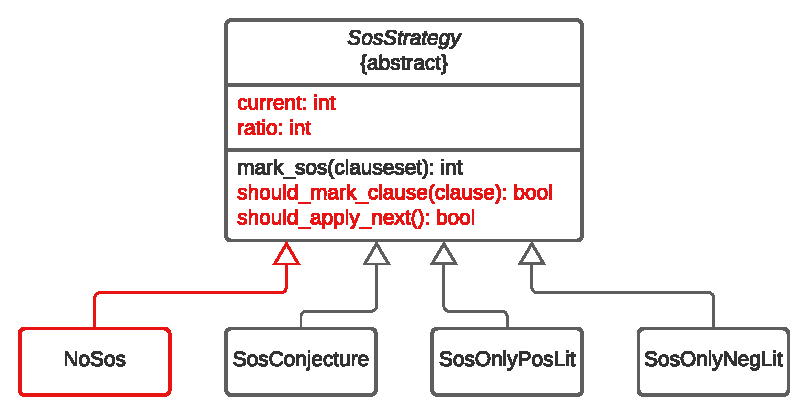
\includegraphics[width=0.7\linewidth]{images/Lucid/SosStrategy1}
	\caption{Neues Klassendiagramm der SOS-Klassen}
	\label{fig:sosstrategy1}
\end{figure}


Die Änderungen und die Gründe für die spezifische Umsetzung werden in den nächsten Abschnitten erläutert. Tabelle \ref{table:difference_sos_classes} enthält eine Übersicht über die Änderungen und eine Referenz zu den zugehörigen Abschnitten.
\begin{table}[h]
	\centering
	\begin{tabular}{|c|l|c|}
		\hline
		Änderung & Beschreibung & Referenz \\
		\hline
		1 & zusätzliche Klasse NoSos & \ref{section:4.1} \\
		\hline
		2 & zusätzliche Methode should\_mark\_sos() & \ref{section:4.2} \\
		\hline
		3 & \cellbreak{l}{zusätzliche Felder current, ratio \\ und zusätzliche Methode should\_apply\_next()} & \ref{section:4.3} \\
		\hline
	\end{tabular}
	\caption{Änderungen zwischen konzeptionellem Klassenkonzept und tatsächlicher Umsetzung}
	\label{table:difference_sos_classes}
\end{table}

\section{Auswahl und Abspeicherung der SOS-Strategie}
\label{section:4.1}

Wie im UML-Diagramm in Abbildung \ref{fig:pyresproofstate} gezeigt ist, gibt es bereits eine Klasse
SearchParams, die für die Speicherung der angewandten Optimierungsstrategien zuständig ist. Die Klasse speichert einfache Optionen wie die Löschung von Tautologien als Wahrheitswert ab. Für komplexere Strategien wie die Heuristiken werden andere Objekte referenziert. Diese setzen eigene Funktionalität um und werden vom Programm aufgerufen.

Die Klasse SearchParams wird so modifiziert, dass sie eine zusätzliche Referenz auf die gewählte SOS-Strategien enthält. Abhängig davon, welche Option der Benutzer wählt, wird eine Instanz einer bestimmten Klasse erzeugt und in SearchParams referenziert. Der Befehl
\begin{lstlisting}
./pyres-fof --set-of-support=Conjecture file.p
\end{lstlisting}
würde zum Beispiel dafür sorgen, dass eine Instanz der Klasse SosConjecture erstellt wird. 
Wenn keine SOS-Strategie angewandt wird, zeigt die Referenz in den SearchParams auf ein Objekt vom Typ NoSos. Dieses Objekt ist als Platzhalter anzusehen. Es ist wie SOSConjecture, SosOnlyPosLit und SosOnlyNegLit von SosStrategy abgeleitet und implementiert alle Methoden. Die Methoden sind allerdings so geschrieben, dass sie beim Aufruf keine Auswirkung auf die Beweissuche haben. Somit wird keine SOS-Strategie angewandt.

Alternativ zu einem Platzhalter-Objekt könnte man die Referenz auch auf None setzen. Dies würde etwas Speicherplatz sparen, hätte jedoch den Nachteil, dass an jeder Stelle im Code, wo eine SOS-Methode aufgerufen wird, vorher geprüft werden müsste, ob das SOS-Objekt existiert. Anderfalls könnte es zu Laufzeitfehlern vergleichbar mit einer Nullpointer-Exception kommen. 

Aus diesem Grund wurde sich für die Einführung des Platzhalter-Objekt entschieden.
\section{Markierung des SOS}
\label{section:4.2}

Das SOS wird einmal vor Beginn der Beweissuche markiert, indem die Methode mark\_sos() aufgerufen wird. Die Methode bekommt die Klauselmenge als Eingabeargument übergeben und iteriert über jede der Klauseln. (siehe Listing \ref{listing:markSos})

\begin{lstlisting}[caption={Methode zur Markierung des SOS}, label={listing:markSos}]
class SosStrategy(object):
	def mark_sos(self, clauseset):
		""" iterates over each clause and in the clauseset and sets part_of_sos to True or False """
		num_sos_clauses = 0
		for clause in clauseset.clauses:
			if self.should_mark_clause(clause):
				clause.part_of_sos = True
				num_sos_clauses += 1
			else:
				clause.part_of_sos = False
		return num_sos_clauses
\end{lstlisting}

Die Methode should\_mark\_clause(), die in Zeile 6 aufgerufen wird, entscheidet, ob die Klausel Teil des SOS sein sollte oder nicht. Abhängig davon wird der Wert von part\_of\_sos auf wahr oder falsch gesetzt.

In der Theorie wäre es möglich, die Funktionalität von should\_mark\_clause() in die Methode mark\_sos() zu intergrieren, sodass es weniger Methoden gibt. Die Auslagerung in eine zusätzliche Methode hat aber zwei Vorteile.
\begin{enumerate}
	\item Getrennte Funktionalität macht den Code lesbarer. mark\_sos() ist lediglich für das Iterieren und das Setzen der Markierung zuständig. Sie delegiert die Entscheidung, ob eine Klausel markiert wird, an eine neue Methode weiter.
	\item Die Methode mark\_sos() kann für alle SOS-Strategien die gleiche Implementierung beibehalten. Lediglich should\_mark\_clause() muss für jede Strategie überschrieben werden.
\end{enumerate}

Die Methoden should\_mark\_clause() sind in Listing \ref{listing:shouldMarkClause} abgebildet.
\begin{lstlisting}[caption={Markierungsmethoden für drei der vier SOS-Strategien. Die Klasse SosOnlyNegLit wurde weggelassen, da sie die gleiche Codestuktur wie SosOnlyPosLit besitzt.}, label={listing:shouldMarkClause}]
class NoSos(SosStrategy):
	def should_mark_clause(self, clause):
		return False

class SosConjecture(SosStrategy):
	def should_mark_clause(self, clause):
		return clause.type == "negated_conjecture"
		
class SosOnlyPosLit(SosStategy):
    def should_mark_clause(self, clause):
		for lit in clause.literals:
			if lit.isNegative():
				return False
		return True
\end{lstlisting}


\section{Implementierung beider Konzepte}
\label{section:4.3}

\paragraph{SOS-Konzept 1: Nicht-SOS zu processed hinzufügen}

Wie im Kapitel Konzeption beschrieben, müssen alle Klauseln, die nicht zum SOS gehören zu den verarbeiteten Klauseln hinzugefügt werden. Diese Aktion muss nach Markierung des SOS und vor Beginn der Beweissuche durchgeführt werden. Zur Übersicht wird eine Methode init\_sos() hinzugefügt, die erst das SOS markiert und danach die Nicht-SOS-Klauseln als verarbeitet festlegt.

\paragraph{SOS-Konzept 2: SOS und Nicht-SOS mit unterschiedlicher Priorität verarbeiten}

Das Verhältnis $r$ mit dem SOS- und Nicht-SOS-Klauseln verarbeitet werden, ist in der Variable ratio der SOS-Klasse abgespeichert. Dieses Verhältnis kann vom Benutzer als Eingabegröße ausgewählt werden (siehe \ref{listing:UserSelectRatio}). Zeile 1 legt kein $r$ fest wodurch automatisch das erste Konzept gewählt wird. Der tatsächliche Wert der Variablen ratio ist dann 0. Zeile 2 setzt ratio auf 3. Zeile 3 ist die Kurzschreibweise für Zeile 2

\begin{lstlisting}[label={listing:UserSelectRatio}]
./pyres-fof --set-of-support=Conjecture file.p
./pyres-fof --set-of-support=Conjecture --sos-ratio=3 file.p
./pyres-fof -OConjecture -R3 file.p
\end{lstlisting}

Der gewählte Wert von $r$ fließt in die Beweissuche mit ein, indem die Methode extractBest() angepasst wird. Bisher floss in die Auswahl der nächsten Klausel lediglich die gewählte Heuristik-Strategie ein, welche eine Klausel anhand von Warteschlangenposition und Symbolanzahl auswählt. 

In die angepasste Methode soll zusätzlich die Information einfließen, welche Klauseln im SOS sind und ob als nächstes eine SOS- oder Nicht-SOS-Klausel gewählt werden soll. Dies wird gemacht, indem von der SOS-Klasse die Methode should\_apply() aufgerufen wird. Sie gibt den Wahr oder Falsch zurück abhängig davon, ob die nächste Klausel im SOS liegen soll oder nicht. Die Implementierung dieser Methode erfolgt über eine interne Zählvariable current.

Ist der Rückgabewert von should\_apply() wahr, dann wird extractBest() eine SOS-Klausel auswählen, andernfalls eine Nicht-SOS-Klausel. Welche SOS-Klausel genau ausgewählt wird, hängt dann von der angewandten Heuristik ab.

Ein Spezialfall muss gesondert behandelt werden. Wird als nächstes eine SOS-Klausel erwartet und die Menge der unverarbeiteten Klauseln enthält nur Nicht-SOS-Klausel, dann werden erneut alle Klauseln durchlaufen und es wird explizit eine Nicht-SOS-Klausel gesucht. Äquivalent wird der Fall behandelt, dass eine Nicht-SOS-Klausel gesucht wird und nur noch SOS-Klauseln vorhanden sind.

\section{weitere Implementierungen}

Auch das 

\paragraph{Vererbung des SOS-Zustands}
Wie in der Konzeption beschrieben, wird eine abgeleitete Klausel zum SOS hinzugefügt, wenn mindestens eine der Eltern-Klauseln Teil des SOS ist. Die entsprechenden Anpassungen im Code sind sehr einfach (siehe Quellcode \ref{listing:InheritSos})
\begin{lstlisting}[caption={Implementierung der Vererbung des SOS.Zustands an abgeleitee Klauseln}label={listing:InheritSos}]
def resolution(clause1, lit1, clause2, lit2):
	...
	res.part_of_sos = clause1.part_of_sos or clause2.part_of_sos
	return res
	
def factor(clause, lit1, lit2):
	...
	res.part_of_sos = clause.part_of_sos
	return res
\end{lstlisting}
Eine weitere Methode, in der eine SOS-Vererbung stattfinden muss, ist bei der Erstellung von Klauselkopien mit neuen Variablen. Diese Aktion wird von der Methode FreshVarCopy() durchgeführt und vor dem Verarbeiten einer einzelnen Klausel aufgerufen.
Im Gegensatz zur Resolution und Faktorisierung enthält FreshVarCopy() keine neuen semantischen Informationsgehalt, sondern wird nur angewandt, um Kollisionen von Variablennamen während der Resolution zu verhindern.


\paragraph{Speicherung der Anzahl von SOS-Klauseln}
Zur Umsetzung der SOS-Strategien ist es nicht nötig, die momentane Anzahl von SOS-Klauseln einer Klauselmenge zu speichern. Die Speicherung vereinfacht aber den Code zur Auswahl der nächsten Klausel, da einfach überprüft werden kann ob es SOS- oder Nicht-SOS-Klauseln in der Klauselmenge gibt (siehe Abbildung \ref{fig:selectnext})

Im ersten Schritt wird festgelegt, ob die nächste Klausel im SOS liegen soll oder nicht. Gibt es keine SOS-Klauseln in der Klauselmenge, dann wird dieser Wert auf falsch gesetzt und gibt es keine Nicht-SOS-Klauseln, dann wird der Wert zwangsweise auf wahr gesetzt. Auf diese Weise ist gewährleistet, dass es immer mindestens eine Klausel gibt, die den SOS-Zustand erfüllt. 

Wenn es sowohl SOS- als auch Nicht-SOS-Klauseln gibt, dann wird die Methode should\_apply() aufgerufen, die den SOS-Zustand für die nächste Klausel bestimmt. Die Funktionsweise dieser Methode wurde bereits in Sektion \ref{section:4.3} erläutert.

In einem zweiten Schritt wird über alle Klauseln der Klauselmenge iteriert. Die Methode sucht diejenige Klausel, die den optimalen Wert nach angewandten Heuristik hat und berücksichtigt nur Klauseln, die den SOS-Zustand aus dem ersten Schritt erfüllen. Die ausgewählte Klausel wird zurückgegeben.

Findet die Methode keine passende Klausel, gibt sie None zurück. Dieser Fall komm nur dann vor, wenn die Klauselmenge leer ist. In der Praxis kann dieses Szenario nicht eintreten, da vor dem Verarbeiten einer Klausel überprüft wird, ob es noch unverarbeitete Klauseln gibt. Sollte die Klauselmenge leer sein, gilt das Problem als erfüllbar und es werden keine Klauseln mehr verarbeitet.

\begin{figure}
	\centering
	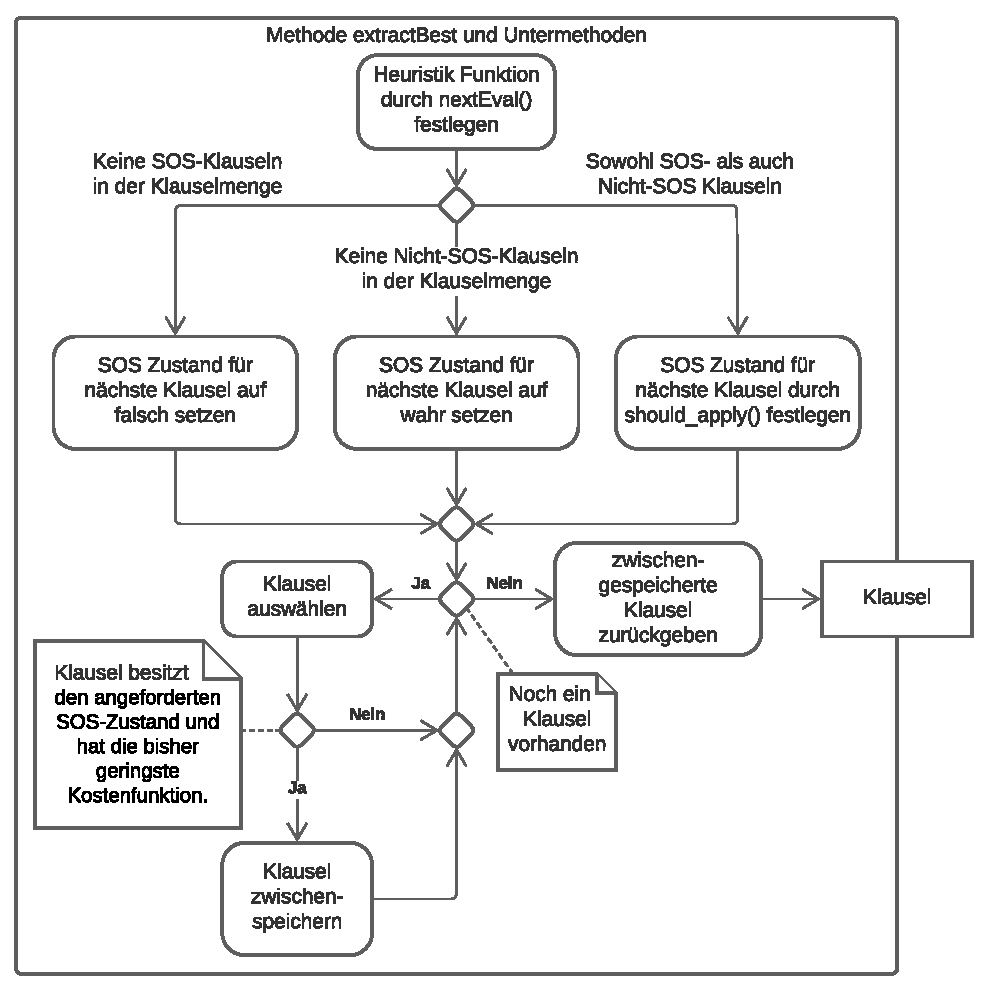
\includegraphics[width=0.9\linewidth]{images/Lucid/SelectNext}
	\caption{Aktivitätsdiagramm für die Auswahl der nächsten Klausel}
	\label{fig:selectnext}
\end{figure}

